\documentclass[conference]{IEEEtran}
\IEEEoverridecommandlockouts
% The preceding line is only needed to identify funding in the first footnote. If that is unneeded, please comment it out.
%----------------------------------------------------------
\usepackage{cite}
\usepackage[pdftex]{graphicx}
% declare the path(s) where your graphic files are
\graphicspath{images/}
\DeclareGraphicsExtensions{.pdf,.jpeg,.png,.jpg}
\usepackage{amsmath,amssymb,amsfonts}
\usepackage{algorithmic}
\usepackage{graphicx}
\usepackage{textcomp}
\usepackage{array}
%\usepackage[caption=false,font=normalsize,labelfont=sf,textfon =sf]{subfig}
\usepackage{dblfloatfix}
\usepackage{url}
\usepackage{lipsum}
\usepackage{listings}
\usepackage{xcolor}
\def\BibTeX{{\rm B\kern-.05em{\sc i\kern-.025em b}\kern-.08em
    T\kern-.1667em\lower.7ex\hbox{E}\kern-.125emX}}
%----------------------------------------------------------
    \lstset{
        escapeinside={/*@}{@*/},
        language=Python,	
        basicstyle=\fontsize{8.5}{12}\selectfont,
        numbers=left,
        numbersep=2pt,    
        xleftmargin=2pt,
        frame=tb,
        columns=fullflexible,
        showstringspaces=false,
        tabsize=4,
        keepspaces=true,
        showtabs=false,
        showspaces=false,
        morekeywords={inline,public,class,private,protected,struct},
        captionpos=b,
        lineskip=-0.4em,
        aboveskip=10pt,
        extendedchars=true,
        breaklines=true,
        prebreak = \raisebox{0ex}[0ex][0ex]{\ensuremath{\hookleftarrow}},
        keywordstyle=\color[rgb]{0,0,1},
        commentstyle=\color[rgb]{0.133,0.545,0.133},
        stringstyle=\color[rgb]{0.627,0.126,0.941},
    }
%----------------------------------------------------------

\begin{document}

\title{Projeto de comunicação serial entre arduinos\\
{\footnotesize \textsuperscript{*} Sistemas Embarcados: Prof. Marco Reis - marco.reis@ba.docente.senai.br}
\thanks{Identify applicable funding agency here. If none, delete this.}
}

% \author{\IEEEauthorblockN{Marco Reis, 41650-010\IEEEauthorrefmark{1}}
% \IEEEauthorblockA{\IEEEauthorrefmark{1}Robotics & Autonomous Systems Center,
% Senai Cimatec, Salvador, Brazil}% <-this % stops an unwanted space


\author{\IEEEauthorblockN{Kauan Dantas Brito da Silva}
\IEEEauthorblockA{\textit{Senai Cimatec} \\
\textit{Engenharia elétrica}\\
Salvador, Bahia, Brasil \\
kauan27dbrito@gmail.com}

}

\maketitle

\begin{abstract}
    The project is carried out on the Tinker cad platform and consists of a serial communication between two 
    arduinos, in which one transmits the information and the other receives it. The first Arduino is composed
    of an ultrasonic sensor that calculates the distance of an object, in addition to indicating the region where
    the object is through colored LEDs. The second arduino is composed of an LCD monitor that receives the
    information given by the first arduino and emits this distance on the screen.
\end{abstract}

\begin{IEEEkeywords}
Project, arduino, build, hardware, software 
\end{IEEEkeywords}

\section{Introdução}
O arduino é um dispositivo eletrônico open source que de acordo com o livro arduino em ação, teve seu inicio na Itália, 
em 2005 no Interaction Design Institute na cidade de Ivrea. Com o intuito de promover um ambiente propício para o
desenvolvimento de novas tecnologias, o professor Massimo Banzi juntamente com um pesquisador visitante denominado
David Cuartielles elaboraram um dispositivo barato e simples de usar, completamente o oposto dos dispositivos 
disponíveis no mercado da época \cite{evans2013}.

Visto isso, análogo aos ideais dos criadores do arduino, o presente artigo tem como intuito agregar conhecimento 
ao estudante que está visando aprender sobre esse equipamento de forma prática, através de um projeto de comunicação 
serial[Fig. 1] entre dois arduinos, via porta TX RX, no qual um dos arduinos transmite a distância de um objeto e o outro 
recebe  essa informação e disponibiliza no display. Com isso, a elaboração desse projeto visa construir e auxiliar o 
desenvolvimento estudantil, seja ele básico, médio ou superior.
%/Fig.~\ref{fig2}.
\begin{figure}[htbp]
    \centerline{
        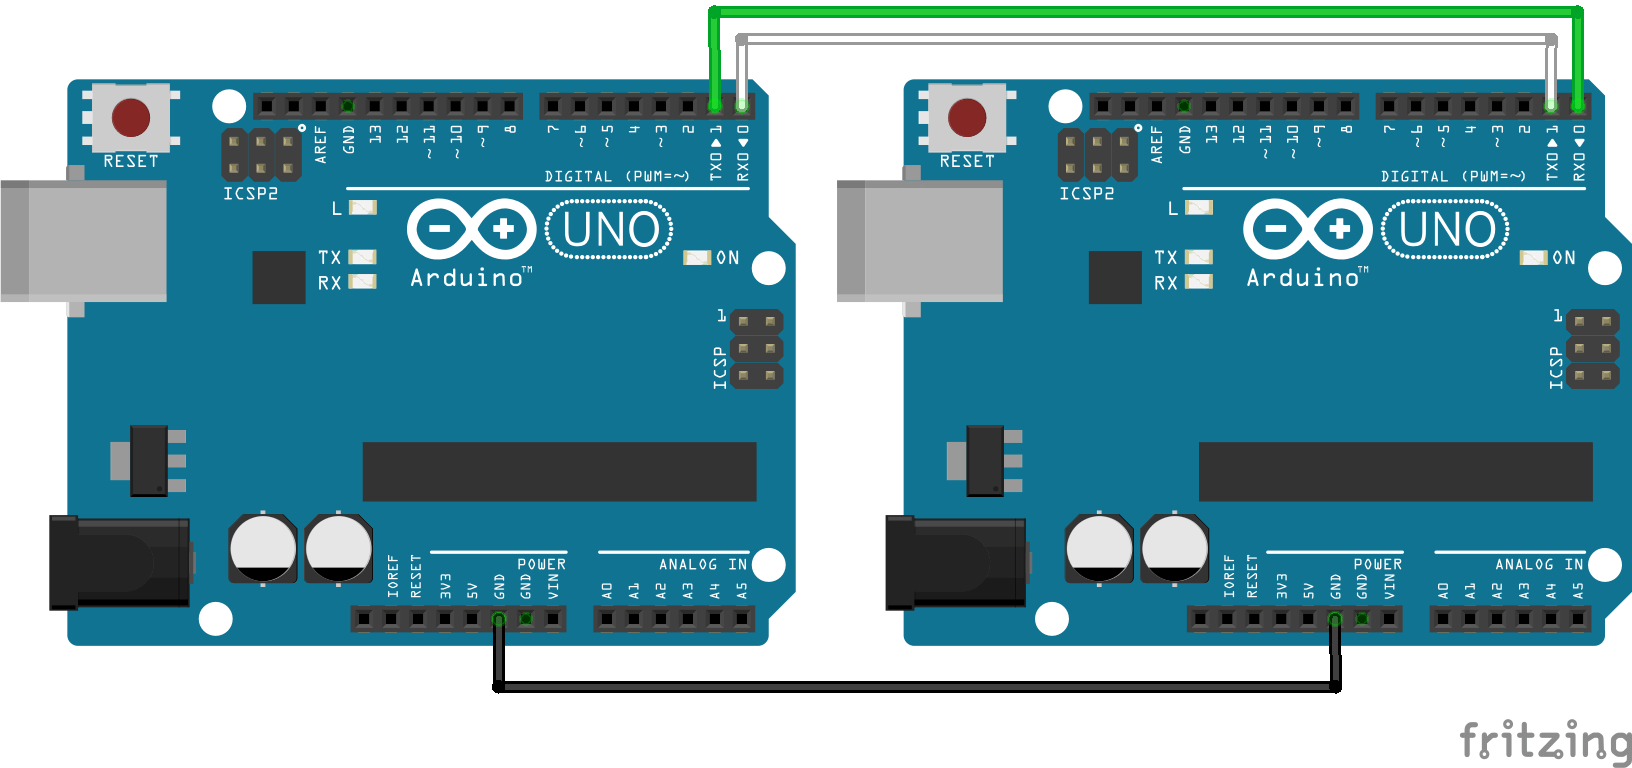
\includegraphics[width=7cm]{images/fig2.png}
        }
    \caption{Comunicação serial \cite{Acomunic15:online}}
    \label{figura:fig2}
    \end{figure}

\section{Desenvolvimento}

\subsection{Materiais}

Hardware:
\begin{itemize}
\item 45 Fios conectores;
\item 3 Leds, vermelho, azul e branco;
\item 3 Resistores de  220 $ \Omega  ; $
\item 2 Arduinos UNO;
\item 2 Protoboards;
\item 1 Resistor de 1 K $\Omega  ; $ 
\item 1 Sensor ultrassônico HC-SR04;
\item 1 Potenciômetro;
\item 1 Display LCD;
\item 1 Computador; 

Software:
\item GitHub;
\item Tinkercad (C); 
\item Visual Studio Code (latex);
\end{itemize}

\subsection{Métodos}
O projeto foi todo realizado na plataforma tinker cad e inicialmente, pesquisou-se como realizaria a conexão do sensor ultrassônico HC-SR04(Fig. 2) e do display LCD 
(Fig. 3) no arduino UNO, através do site do How to Mechatronics, a partir disso foi realizada programação dos 
mesmos, atribuindo seus parâmetros e configuração de portas, conforme o código do anexo 1 que localiza a programação 
do sensor e  o anexo 2, a programação do display. Posteriormente foi realizada a comunicação serial, usando o 
protocolo de comunicação assíncrono UART, na qual é feita uma conexão física entre duas portas do arduino, uma 
denominada RX que é responsável pela recepção da informação e a TX que transmite a informação (Fig. 1).
 %/Fig.~\ref{fig2}., %/Fig.~\ref{fig3}., anexo 1 e 2

 \begin{figure}[htbp]
    \centerline{
        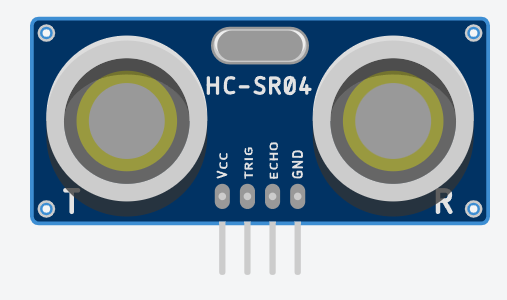
\includegraphics[width=4.5cm]{images/fig3.PNG}
        }
    \caption{Sensor ultrassônico HC-SR04 [própria]}
    \label{figura:fig3}
    \end{figure}

    \begin{figure}[htbp]
        \centerline{
            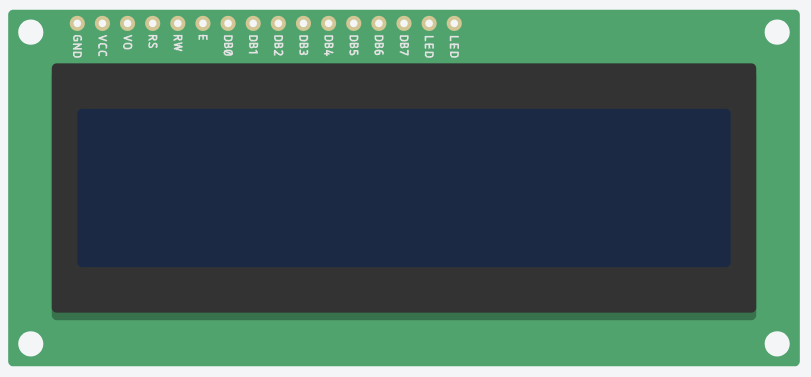
\includegraphics[width=4.5cm]{images/fig4.PNG}
            }
        \caption{Display LCD [própria]}
        \label{figura:fig4}
        \end{figure}

 Em seguida foi realizado a conexão dos leds, com seus devidos resistores de 220 $\Omega$ (Fig. 4) e sua definição
 de parâmetros, bem como sua programação para localizar as regiões(Fig. 5), divididas em: Região 1, de 0 a 112 cm
 o led vermelho acende, região 2 de 112 a 223cm o led azul ascende e de 223 a 355 o led branco ascende.
 %/Fig.~\ref{fig4} e anexo 3

 \begin{figure}[htbp]
    \centerline{
        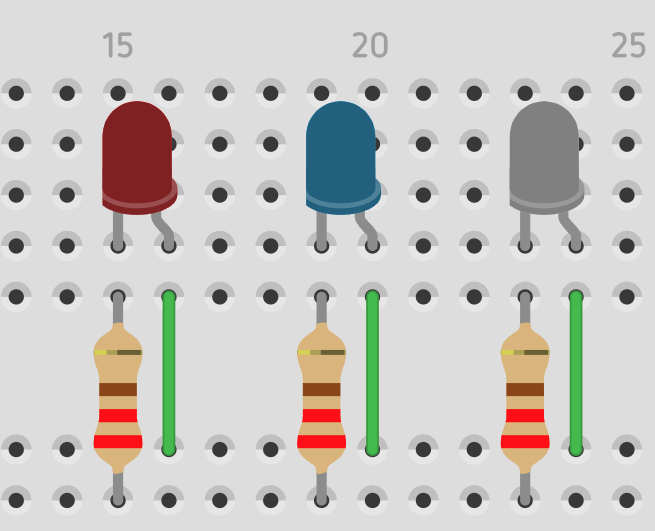
\includegraphics[width=4.5cm]{images/fig5.PNG}
        }
    \caption{leds e resistores de 220 $\Omega$ [própria]}
    \label{figura:fig5}
    \end{figure}

    \begin{figure}[htbp]
        \centerline{
            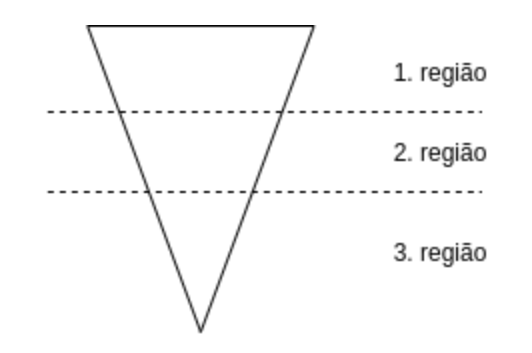
\includegraphics[width=5cm]{images/fig6.PNG}
            }
        \caption{Divisão das regiões [desconhecida]}
        \label{figura:fig6}
        \end{figure}
Por fim, juntando essas partes e colocando o código no github para o versionamento do mesmo, no qual subsequentemente o projeto foi desenvolvido como um todo e dessa forma gerando um circuito final (Fig. 7). Logo após
foi realizado o artigo no Vs Code usando a linguagem latex.

\begin{figure}[htbp]
    \centerline{
        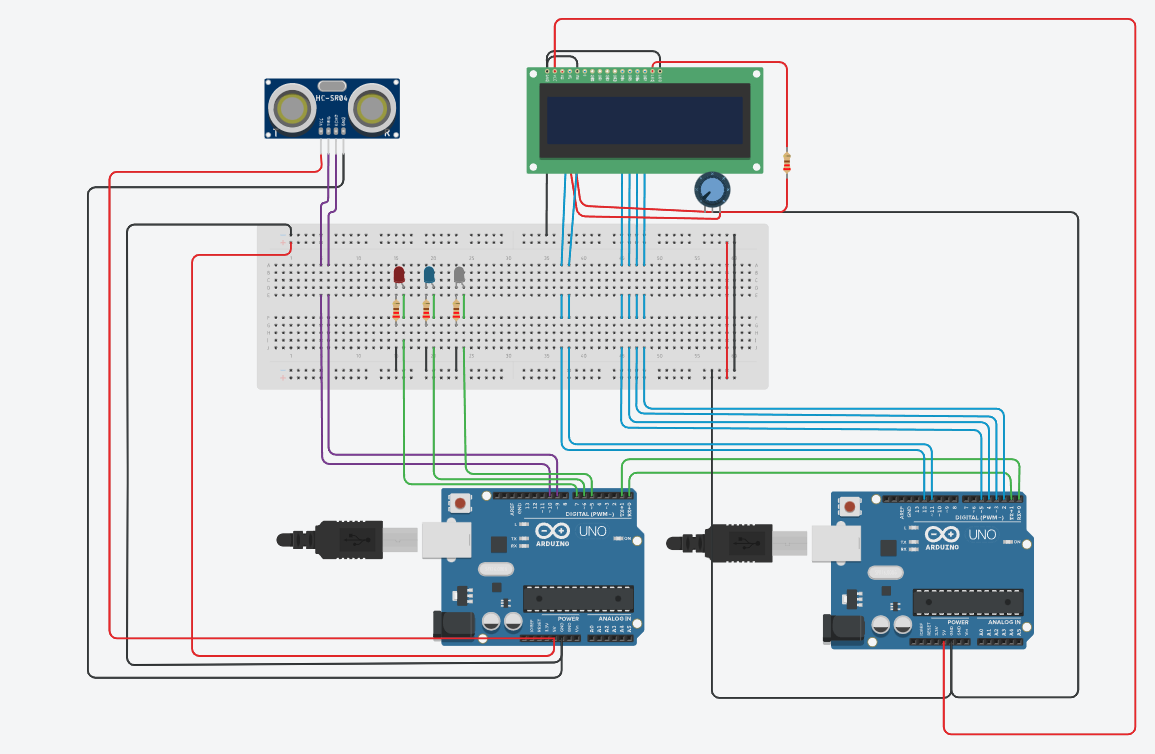
\includegraphics[width=8cm]{images/fig7.PNG}
        }
    \caption{Ciruito completo [própria]}
    \label{figura:fig6}
    \end{figure}


\section*{Conclusão}
Neste trabalho foi possível demonstrar a comunicação entre dois arduinos e seus respectivos componentes, com a finalidade de criar 
uma nova aplicação explicativa que consiste na recepção de dados por um dispositivo e a recepeção por outro equipamento. 

Portanto, é notório observar como se comporta e se aplica a comunicação serial, onde suas 
funcionalidades abre um leque de possiblidades para projetos distintos. Não necessitando assim, configurar todo o projeto com um
único Arduino, gerando uma variedade bastante ampla para disversas aplicações. Desta maneira, proporcionando o senso de curiosidade no leitor,
fazendo-o refazer o esquema estrurado ao longo do artigo.

Dessa forma,cumprindo o objetivo do presente artigo que é desenvolver estudantes, atiçando a vontade de descobrir algo novo ou
de desevolver uma melhoria, o fato é, quando o ser humano entende minimamente algo em que gosta, ele é capaz de buscar mais e mais
o conheciemento necesário para evoluir seu conhecimento acerca do obejeto de estudo.  


%----------------------------------------------------------
\bibliographystyle{IEEEtran}
\bibliography{Bibliography}
%CRITICAL: do not change the above two lines!!!
%----------------------------------------------------------

\end{document}
